\documentclass{llncs}


\usepackage{hyperref}
\usepackage{graphicx}
\usepackage{multirow}
\usepackage[misc,geometry]{ifsym}

\usepackage{amsmath}
\usepackage{enumitem}
%\usepackage{amsfonts}
%\usepackage{amssymb}
%\usepackage{epstopdf}
%\usepackage{epsfig}

%\usepackage[utf8x]{inputenc}
%\usepackage[english,russian]{babel}



\begin{document}

\mainmatter 

\title{Parallel Global Optimization for Non-Convex Mixed-Integer Problems
\thanks{This study was supported by the Russian Science Foundation, 
project No.\,16-11-10150.}}
\author{Konstantin Barkalov \and Ilya Lebedev %\Letter 
\\
\email{ \{konstantin.barkalov,ilya.lebedev\}@itmm.unn.ru}}

\institute{
Lobachevsky State University of Nizhni Novgorod, Nizhni Novgorod, Russia
}

\maketitle

\begin{abstract}

The paper considers the mixed-integer global optimization problems. A novel 
parallel algorithm for solving the problems of this class based on the index 
algorithm to solving the continuous global optimization problems has been proposed. 
The comparison of this algorithm with known analogs demonstrates the efficiency of the 
developed approach. 
%Russian
The proposed algorithm allows an efficient parallelization including the employment of the 
graphics accelerators. The results of performed numerical experiments (solving a series of 100 multiextremal mixed-integer problems) confirm a good speedup of the algorithm with the use of GPU. 

\keywords global optimization, non-convex constraints, mixed-integer problems.

\end{abstract}

\section{Introduction}\label{sec:intro}

In this paper the global optimization problems and the method of solving these ones are 
considered. The global optimization problems are the time-consuming ones since the global 
optimum is an integral characteristic of the problem being solved and requires the investigation 
of the whole search domain. 
As a result, the search of the global optimum is reduced to the construction of a coverage (in 
general, a nonuniform one) of the space of parameters. 
The problems, in which some parameters can take the discrete or integer values only (mixed-integer global 
optimization problems) are of special interest because for these problems it is more difficult to build 
the estimates of the optimum as compared to the continuous ones.

The situation when some parameters are featured by the discreteness or integerness is frequent 
in applied problems. As a rule, the integer parameters take a small number of values and may 
denote, for example, the trademarks of the materials used, the variant of typical layouts of 
components, etc.

A lot of publication have been devoted to the methods of solving the mixed-integer problems 
(see, for example, the reviews~\cite{Burer,Boukouvala}). The well known deterministic 
methods of solving the problems of this class are based, as a rule, on the Branch-and-Bound 
\cite{Belotti} or on the Branch-and-Reduce approach \cite{Vigerske}. Also, a number of 
the metaheuristic and genetic 
algorithms are known, which are based one way or another on the random search concept 
\cite{Deep,Schluter}.

In the present study, we proposed a novel parallel method for solving the mixed-integer 
problems based on the index approach to solving the constrained global optimization 
problems \cite{Strongin2000,Strongin2013}. 
%Russian
Within the framework of this approach: 
\begin{itemize}
	\item 
	the solving of the multidimensional problems is reduced to solving the equivalent one-dimensional problems; the corresponding reduction is based on the use of the space-filling curves;
	\item 
	when solving the constrained optimization problems, each constraint is taken into 
account and processed separately, the penalty functions are not used;
	\item 
	the parallelization of the search process is performed by means of the simultaneous 
computing of several objective function values at different points of the search domain within 
every iteration.
\end{itemize}

The paper text reflecting the results of the performed study is organized in the following way. 
In Section 2, a brief description of the dimensionality reduction scheme using the space-filling 
curves is given. Also, the index scheme of accounting for the constraints is described. Here the 
formulation of the parallel index algorithm for solving the continuous global optimization 
problems is given as well.
In Section 3, the approach to the generalization of the parallel index algorithm with the purpose 
of solving the mixed-integer problems is presented. A method that allows to reduce solving of 
mixed-integer problem to solving a set of the continuous optimization problems, which can be 
performed in parallel, is given. 
Section 4 contains the results of numerical experiments. The comparison of the sequential 
version of the algorithm with the known analogs is conducted here. Also, the efficiency of the 
parallel CPU- and GPU-versions of the algorithm for solving a series of the multiextremal 
mixed-integer problem is demonstrated. 
Section 5 concludes the paper.


\section{Global optimization algorithm and dimension reduction}

A constrained global optimization problem can be formulated as follows
%Let us consider the $N$-dimensional global optimization problem
\begin{gather}\label{problem}
\varphi(y^\ast)=\min{\left\{\varphi(y):y\in D, \; g_i(y)\leq 0, \; 1 \leq i \leq m\right\}},\\
D=\left\{y\in R^N: a_j\leq y_j \leq b_j, 1\leq j \leq N \right\}.\label{D}
\end{gather}
The objective function $\varphi(y)$ (hereafter denoted by $g_{m+1}(y)$) and the left-hand 
sides $g_i(y), \; 1\leq i \leq m,$ of the constraints satisfy the Lipschitz condition 
\[
\left|g_i(y_1)-g_i(y_2)\right|\leq L_i\left\|y_1-y_2\right\|, \;1\leq i\leq m+1, \; y_1,y_2 \in D,\;
\]
with a priori unknown constants $L_i, \; 1 \leq i \leq m+1,$ and may be multiextremal. It is 
assumed that the functions $g_i(y)$ are defined and computable only at the points $y \in D$ 
satisfying the conditions
\begin{equation}\label{g_k}
g_k(y) \leq 0, \; 1 \leq k < i.
\end{equation}

By employing the continuous single-valued Peano-Hilbert curve $y(x)$ mapping the unit 
interval 
$[0,1]$ on the $x$-axis onto the $N$-dimensional domain (\ref{D}), it is possible to find the 
minimum in (\ref{problem}) by solving the one-dimensional problem
\[
\varphi(y(x^\ast))=\min \left\{\varphi(y(x)): x \in [0,1], \; g_i(y(x))\leq 0, \; 1 \leq i \leq m\right\}.
\]
Algorithms for numerical construction of Peano-Hilbert curve approximation (\textit{evolvent}) are 
considered in \cite{Strongin2000,Strongin2013}. These evolvents are fractals generated by an iterative
process, that fill in the hypercube $D$ with accuracy $2^{-m}$, where integer $m>0$ is the 
evolvent construction parameter. Examples of the evolvent with different $m$ in two dimensions are given in Fig.~\ref{evolvents}.

\begin{figure}
\begin{minipage}{0.49\linewidth}
\center{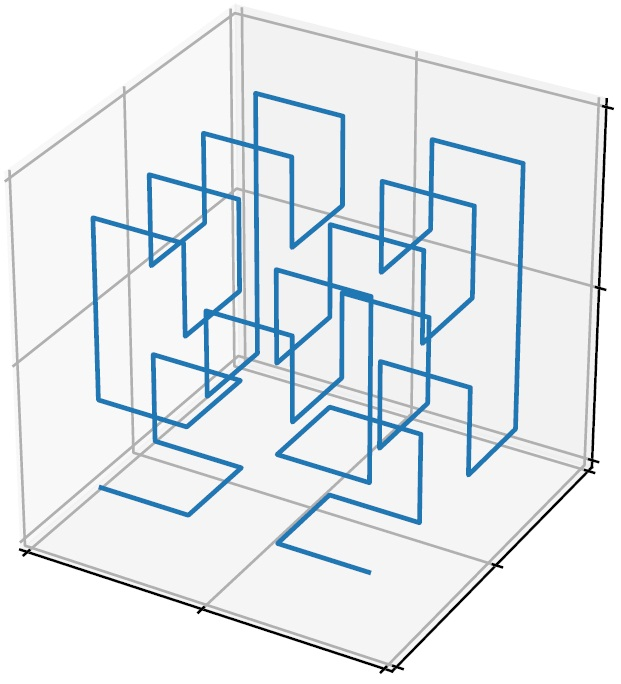
\includegraphics[width=1.0\linewidth]{fig1b.JPG} \\ (a)}
\end{minipage}
\begin{minipage}{0.49\linewidth}
\center{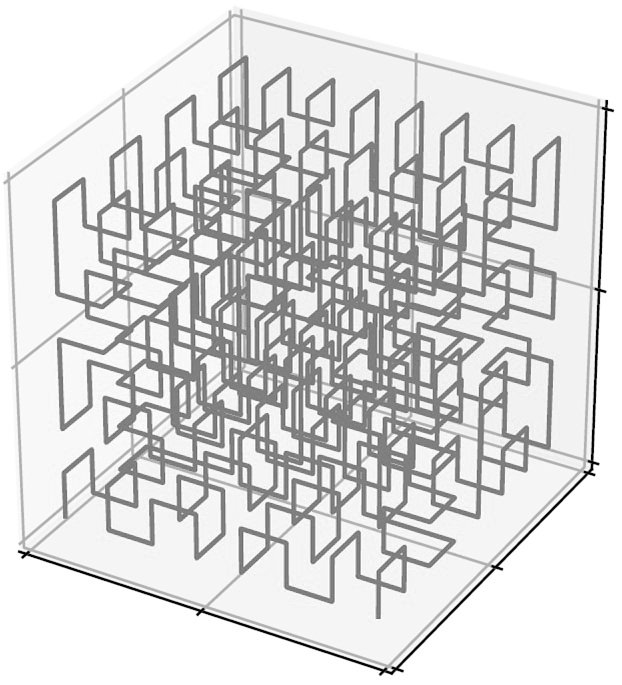
\includegraphics[width=1.0\linewidth]{fig1c.JPG} \\ (b)}
\end{minipage}
\caption{Evolvents in two dimensions with (a) $m=4$ and (b) $m=5$}
\label{evolvents}
\end{figure}


Due to (\ref{g_k}) the functions $g_i(y(x))$ are defined 
and computable in the subranges 
\[
Q_1=[0,1], \; Q_{i+1}=\left\{x \in Q_i : g_i(y(x)) \leq 0 \right\}, \; 1 \leq i \leq m.
\]

These conditions allows us to introduce a classification of the points $x \in [0,1]$ according to 
the number $\nu (x)$ of the constraints computed at this point. The \textit{index} $\nu(x)$ can 
also be defined by the conditions
\begin{equation}\label{nu}
g_i(y(x)) \leq 0, \; 1 \leq i < \nu, \; g_\nu(y(x))>0,
\end{equation}
where the last inequality is inessential if $\nu=m+1$.

In the dimensionality reduction scheme considered here, a multidimensional problem with 
Lipschitzian functions is juxtaposed with a one-dimensional problem, where the corresponding 
functions satisfy uniform H{\"o}lder condition (see \cite{Strongin2013}), i.e.,
\[
\left|g_i(y(x_1))-g_i (y(x_2))\right| \leq H_i \left|x_1-x_2 \right|^{1/N}, \; x_1,x_2\in [0,1], \; 
1\leq i \leq m+1.
\]
Here, $N$ is the dimensionality of the initial multidimensional problem and the coefficients 
$H_i$ are related to the Lipschitz constant $L_i$ of the initial problem as $H_i \leq 2L_i 
\sqrt{N+3}$.

Thus, \textit{a trial} at a point $x^k \in [0,1]$ executed at the $k$-th iteration of the algorithm 
will consist of the following sequence of operations:
\begin{itemize}
	\item Determine the \textit{image} $y^k=y(x^k)$ in accordance with the mapping 
$y(x)$;
	\item Compute the values $g_1(y^k),..., g_\nu(y^k),$ where $\nu = \nu(x^k)$ is from 
(\ref{nu}). 
\end{itemize}
The dyad 
\begin{equation} \label{trial_result}
 \{ \nu=\nu(x^k), \; z^k=g_\nu(y(x^k)) \} 
\end{equation}
will be referred to as the \textit{trial outcome}.

An efficient parallel index algorithm (PIA) for solving the constrained global optimization 
problem (\ref{problem}) has been developed at University of Nizhni Novgorod. The scheme of 
the algorithm is as follows.

Suppose we have $p \geq 1$  computational elements (e.g., processor cores), which can be 
used to run $p$ trials simultaneously. In the first iteration of the method, $p$ trials are run in 
parallel at various random points $x^i\in(0,1)$, $1\leq i \leq p$. 
Suppose $n \geq 1$  iterations of the method have been completed, and as a result of which, 
trials were carried out in $k=k(n)$ points $x^i, 1\leq i \leq k$. Then the points 
$x^{k+1},...,x^{k+p}$  of the search trials in the next $(n+1)$-th iteration will be determined 
according to the rules below.

\begin{enumerate}
\item 
Renumber the points $x^1,...,x^k$ from previous iterations with lower indices, lowest to highest 
coordinate values, i.e.
\begin{equation}\label{Eq:17}
0=x_0<x_1<...<x_i<...<x_k<x_{k+1}=1,
\end{equation}
and match them with the values $z_i=g_\nu(y(x_i))$, $\nu=\nu(x_i)$, $1 \leq i \leq k$, from 
(\ref{trial_result}), calculated at these points; points $x_0=0$ and $x_{k+1}=1$ are introduced 
additionally, the values $z_0$ and $z_{k+1}$ are indeterminate.
\item
Classify the numbers $i,1\leq i \leq k$, of the trial points from (\ref{Eq:17}) by the number of 
problem constraints fulfilled at these points, by building the sets
\begin{equation}\label{Eq:18}
I_\nu = \left\{i: 1 \leq i \leq k,\ \nu = \nu(x_i)\right\},\ 1 \leq \nu \leq m+1,
\end{equation}
containing the numbers of all points $x_i,1\leq i \leq k$, with the same values of $\nu$. The end 
points $x_0=0$ and $x_{k+1}=1$ are interpreted as those with zero indices, and they are 
matched to an additional set $I_0= \left\{ 0,k+1 \right\}$. 

Identify the maximum current value of the index
\begin{equation}\label{Eq:19}
M=\max \left\{\nu = \nu(x_i), \ 1\leq i \leq k\right\}.
\end{equation}
\item
For all values of $\nu, \ 1\leq \nu \leq m+1$, calculate the values  
\begin{equation}\label{Eq:20}
\mu_\nu = \max \left\{ \frac{\left|z_i-z_j\right|}{\left(x_i-x_j\right)^{1/N}} : i,j \in I_\nu, 
j<i\right\}.
\end{equation}
If the set $I_\nu$ contains less than two elements or $\mu_\nu$ from (\ref{Eq:20}) equals zero, 
then assume $\mu_\nu=1$.
\item
For all non-empty sets $I_\nu$, $1 \leq \nu \leq m+1$, determine the values
\begin{equation}\label{Eq:21}
  z^\ast_\nu =  
   \begin{cases}
    -\epsilon_\nu,  \nu < M, \\
    \min{\left\{g_\nu(x_i):i\in I_\nu\right\}}, \nu = M,
   \end{cases}
\end{equation}
where $M$ is the maximum current value of the index, and the vector $\epsilon _R=\left(\epsilon_1,...,\epsilon_m\right)$ with positive coordinates is called the \textit{reserve vector} and is used as a parameter in the 
algorithm.
\item
For each interval $(x_{i-1},x_i)$,$1 \leq i \leq k+1$, calculate the \textit{characteristic} $R(i)$: 
\[
R(i)=\Delta_i+ \frac{(z_i-z_{i-1})^2}{(r_\nu\mu_\nu)^2\Delta_i}-2\frac{z_i+z_{i-1}-
2z^\ast_\nu}{r_\nu\mu_\nu},\;\; \nu=\nu(x_{i-1})=\nu(x_i),
\]
\[
R(i)= 2\Delta_i-4\frac{z_i-z^\ast_\nu}{r_\nu\mu_\nu},\;\; \nu(x_{i-1})<\nu(x_i)=\nu,
\]
\[
R(i)= 2\Delta_i-4\frac{z_{i-1}-z^\ast_\nu}{r_\nu\mu_\nu},\;\; \nu = \nu(x_{i-1})>\nu(x_i).
\]
where $\Delta_i=(x_i-x_{i-1})^{1/N}$, and the values $r_\nu>1, 1\leq\nu\leq m+1$, are used as 
parameters in the algorithm.
\item
Reorder the characteristics $R(i)$, $1\leq i \leq k+1$, from highest to lowest 	
\begin{equation}\label{Eq:23}
R(t_1)\geq R(t_2)\geq ... \geq R(t_{k})\geq R(t_{k+1})
\end{equation}
and choose $p$ largest characteristics with interval numbers $t_j, 1\leq j \leq p$.
\item
Carry out $p$ new trials in parallel at the points $x^{k+j}, 1 \leq j \leq p$, calculated by the 
formulae
\begin{eqnarray*}
& x^{k+j}=\frac{x_{t_j}+x_{t_j-1}}{2}, \; \nu(x_{t_j-1})\neq \nu(x_{t_j}), \\
& x^{k+j}=\frac{x_{t_j}+x_{t_j-1}}{2}- \frac{\mathrm{sign}(z_{t_j}-z_{t_j-
1})}{2r_\nu}\left[\frac{\left|z_{t_j}-z_{t_j-1}\right|}{\mu_\nu}\right]^N, \; \nu(x_{t_j-
1})=\nu(x_{t_j})=\nu. \\
\end{eqnarray*} 

\end{enumerate}

The algorithm stops if the condition $\Delta_{t_j}\leq \epsilon$ becomes true for at least one 
number $t_j, 1\leq j \leq p$; here  $\epsilon>0$ has an order of magnitude of the desired 
coordinate accuracy.

This method of organizing parallel computing has the following justification.
The characteristics of intervals $R(i)$ used in the index algorithm can be considered as
probability measures of the global minimum point location in these intervals. Inequalities
(\ref{Eq:23}) arrange intervals according to their characteristics, and trials are carried out in parallel in
the first $p$ intervals with the largest probabilities.
A detailed description of the algorithm convergence theory is presented in \cite{Strongin2000}.

\section{Parallel algorithm for mixed-integer problems}
%Russian
Now let us consider the case when the argument of the problem functions consists of two 
components: the vector $y$ from the hyperinterval $D$ and the vector $u$ taking a finite 
(and not too large) set of possible values, i.e. 
\begin{gather}\label{problem_i}
\min{\left\{ g_{m+1}(y,u):y\in D, \; g_i(y,u)\leq 0, \; 1 \leq i \leq m\right\}},\\
D=\left\{a_j\leq y_j \leq b_j, \; 1\leq j \leq N \right\}.\nonumber
\end{gather}

Such finite sets can characterize, for example, the variant of material, which the object is made 
from, the geometric sizes, or other quantities, which can belong to a standard discrete series, etc. 

Let us number by the integer values $s, 1\leq s \leq S,$ all possible values of the vector $u$, i.e. 
juxtapose each considered value $s$ with the vector $u_s$. 
Then, the considered problem can be written in the form 
\begin{gather}\label{problem_is}
 \min_{s\in\{1,...,S\}} \left\{ \min_{}{\left\{ g_{m+1}(y,u_s):y\in D, \; g_i(y,u_s)\leq 0, \; 1 \leq i \leq 
m\right\}}\right\},\\
D=\left\{ a_j\leq y_j \leq b_j, \; 1 \leq j\leq N \right\}.\nonumber 
\end{gather}

Using the dimensionality reduction scheme with the evolvent $y(x), x\in [0,1]$, one can 
superimpose each nested minimization problem with respect to $y$ to a one-dimensional 
problem 
\[
 \min{\left\{ g_{m+1}(y(x),u_s):x \in [0,1], \; g_i(y(x),u_s)\leq 0, \; 1 \leq i \leq m\right\}}, 
s\in\{1,...,S\}.
\]

Now let us consider the relation 
\[
Y(x)=y(x-E(x)), \; x\in[0,S],
\]
mapping any point of the interval [0,S] onto the domain $D$ (the notation $E(x)$ corresponds 
to the integer part of the number $x$) and define the functions 
\[
g_i(x) = g_i(Y(x),u_{E(x)+1}), x\in[0,S],
\]
having, in general, the jump discontinuities at the integer points $x_k = i, 1\leq i \leq 
S-1$.
The values $z_k = g_\nu(y(x_k))$ from (\ref{trial_result}) at these points will be considered to 
be undefined, and the values of the indices -- to equal to 0, i.e. $\nu(x_k) = 0$.

Using the introduced notations, one can reformulate the original problem as
\begin{equation}\label{problem_is1}
\min \left\{g_{m+1}(x): x \in [0,S], \; g_i(x) \leq 0, \; 1 \leq i \leq m\right\}.
\end{equation}

As an illustration, Fig. \ref{fig:1} presents the plots of the functions corresponding to a 
problem 
\[
%\min{\left\{ x^2 - 10\cos(2\pi x) + u^2 - 10\cos(2\pi u) : x\in [-2.22, 1.8], u \in {0,1} \right\}}
\min{\left\{ u^2 (\sin(x) +\sin(10x/3) : x\in [2.7, 7.5], u \in \{1,2\} \right\}}
\]
with one continuous parameter $x$ and one binary parameter $u$.
%Еще один график?   

\begin{figure}[ht]
    \centering
    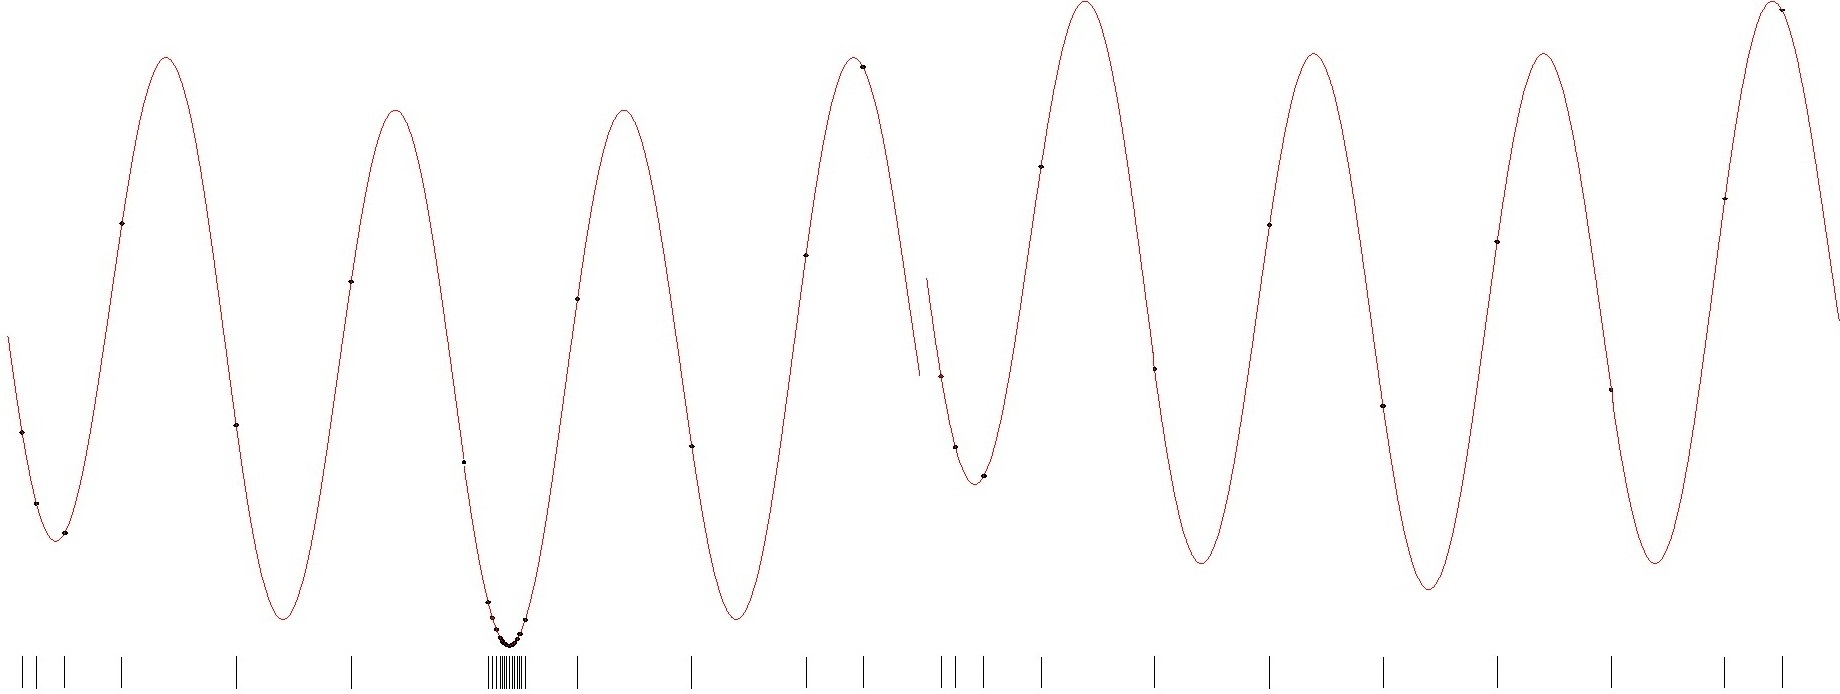
\includegraphics[width=1.0\textwidth] {fig1.jpg}
    \caption{Reduced mixed-integer global optimization problem}
    \label{fig:1}
\end{figure}

Applying the parallel index algorithm to solving the problem (\ref{problem_is1}), we will find 
the solution of the problem (\ref{problem_i}). In this case the major part of trials will conducted 
in 
the subproblem, the solving of which corresponds to the solving of the initial 
problem (\ref{problem_i}). In the rest subproblems, only the minor part of trials will be 
performed 
since the solutions of these subproblems are the locally optimal ones.
%with respect to the solution of the $s$-th subproblem. 
All the above is confirmed by Fig. \ref{fig:1}, where the  
points of trials executed in the course of solving this problem are denoted by the dashes.


Thus, we have constructed the \textit{Mixed-Integer Parallel Index Algorithm} \break 
(MIPIA) based on the  reduction of the mixed-integer non-convex optimization problem to the non-convex optimization problem. 
%Russian
The proposed computational scheme is based on the parallel index method for solving the 
continuous optimization problems and is not oriented onto any particular computational device. 
Here the parallel performing of several trials at different points of the search domain is one of 
key operations (see Step 7 of the algorithm), which can be implemented on CPU (with the use 
of OpenMP and/or MPI) as well as on GPU (with the use CUDA). The issues of the use of 
GPU for these purposes have been considered in details in 
\cite{Barkalov2016,Gergel2016}. This approach to the use of GPU has been applied in 
the implementation of the MIPIA algorithm as well.


\section{Results of experiments}
%Russian
The first series of experiments was conducted using the sequential version of the proposed 
algorithm in order to compare this one with well known methods of similar purpose.

Let us compare proposed MIPIA with a genetic algorithm for solving the mixed-integer global 
optimization problems implemented in Matlab Global Optimization Toolbox \cite{Matlab}. In 
Table \ref{tab:1}, the numbers of trials required for solving the known test mixed-integer 
problems by these methods are presented. For both methods, the same accuracy of search 
$10^{-2}$ were used. These numerical experiments were conducted on a 
computer with Intel Core i5-7300 2.5 GHz processor and 8 Gb RAM under MS Windows 10. 
The results of experiments have demonstrated the advantage of MIPIA in the number 
of iterations as well as in the execution time.

\begin{table}
	\caption{Comparison of MIPIA and GA}
	\label{tab:1}
	\center
	\begin{tabular}{cccccc}
		\hline\noalign{\smallskip}
	\multirow{2}{*}{Test problem}	 & \multicolumn{2}{c}{ GA } & & 
\multicolumn{2}{c}{MIPIA} \\
		\noalign{\smallskip} \cline{2-3} \cline{5-6} \noalign{\smallskip}
		 & $k$ & $t$ & & $k$ & $t$  \\
		\noalign{\smallskip} \hline \noalign{\smallskip}
		 Problem 2 \cite{Floudas}&	481 &	0.0601 & &	417 &	0.04 \\
		 Problem 3 \cite{Floudas}& 	1821 &	0.1130 & & 3324 &	0.107 \\
		 Problem 6 \cite{Floudas}&	641 &	0.0510 & &	118 &	0.001 \\
		 Problem 1 \cite{Deep}   &	481 &	0.1378 & &	66 &	0.0007 \\
		 Problem 2 \cite{Deep}   &	481 &	0.0473 & &	57 &	0.0006 \\
		 Problem 7 \cite{Deep}   &	841 &	0.0736 & & 372	 &	0.017 \\
		\noalign{\smallskip}\hline
	\end{tabular}
\end{table}

The next series of experiments were performed in order to evaluate the speedup of the parallel 
version of the proposed MIPIA algorithm with the use of CPU as well as GPU. In these 
experiments, a series of 100 mixed-integer test problems generated in a random way was solved. 
Computational experiments were carried out on Lobachevsky supercomputer. The node of 
supercomputer included two Intel Sandy Bridge E5-2660 2.2 GHz CPUs and 64 Gb RAM. The 
CPU had 8 cores, i.e. each node had a total of 16 cores and two NVIDIA Kepler K20X GPUs. 

GKLS~\cite{Gaviano} is a well known generator of the test problems for the continuous multiextremal 
optimization. It allows generating the functions of arbitrary dimensionality with 
known properties (the number of local minima, the size of their domains of attraction, the global 
minimizer, etc.).  
This generator of multiextremal functions is often used for the investigations of the global 
optimization algorithms ~\cite{Paulavicius2014,SergeyevKvasov2015,Lebedev2015,Gergel2015}. 
In Fig.~\ref{example} (a) and (b), the contour plots of two-dimensional GKLS functions are 
presented. Figures also shows the points of the trials performed by the method until the required 
accuracy $\epsilon=10^{-2}$ was achieved.

\begin{figure}
\begin{minipage}{0.5\linewidth}
\center{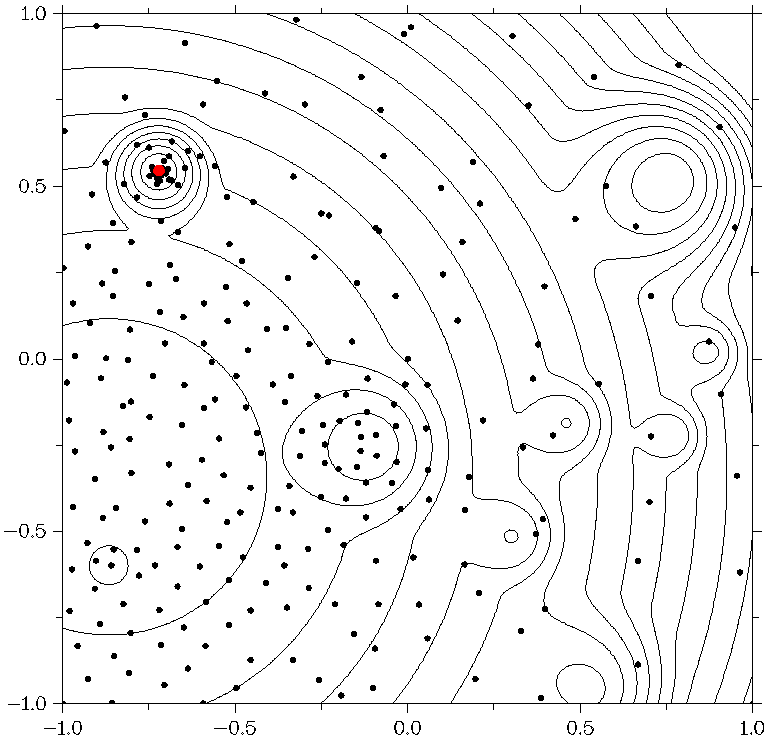
\includegraphics[width=1.0\linewidth]{GKLS-4.png} \\ (a)}
\end{minipage}
\hfill
\begin{minipage}{0.5\linewidth}
\center{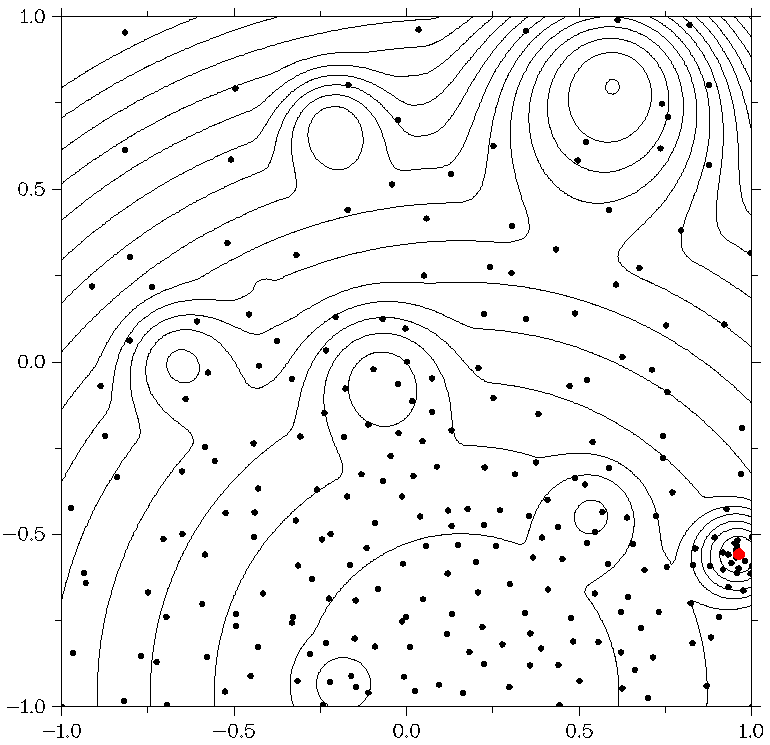
\includegraphics[width=1.0\linewidth]{GKLS-6.png} \\ (b)}
\end{minipage}
\caption{Solving a two-dimensional problem using the index algorithm}
\label{example}
\end{figure}

In the performed experiments, the GKLS generator was used as a base for the construction the 
mixed-integer problems. The rules allowing generating the test problems of this type consist in 
the following.

\begin{enumerate}
	\item A continuous multiextremal function $\varphi(y), y\in D = \left\{ a_j\leq 
y_j\leq b_j, 1\leq j \leq N \right\}$ is generated with the use of the GKLS generator. The global 
minimum of this function is achieved at the known point $y'=(y'_1,...,y'_N)$ and equals 
$\varphi(y')=-1$.
	\item A concave mixed-integer function 
	\[
			h(y,u) = -2 \left[ \sum_{j=1}^N \left( \frac{y_j - y'_j}{b_j-a_j} 
\right)^2 + \sum_{j=1}^M \left( \frac{u_j - b_j}{b_j-a_j} \right)^2 \right],
	\]
	is generated where 
	\begin{gather}
	y\in D = \left\{ a_j\leq y_j\leq b_j, 1\leq j \leq N \right\} \subset R^N,\nonumber \\
	u\in U = \left\{ u_j \in  \left\{a_j, ..., b_j \right\}, 1\leq j \leq M \right\}.\nonumber
	\end{gather}
	This function has $N$ continuous and $M$ discrete parameters and achieves its 
minimum value at the point $(y',b)$.
	\item The coefficient 
	\[
	h_{min} = 4 - \min_{y,u} \left\{ h(y,u) \right\}, \; y\in D, u \in U.
	\]
	is computed. 
It is obvious, that the minimum of a concave function $\mu(y,u)$ is located at one of the corner 
points of the search domain. Therefore, if the problem dimensionality is of the order of 10 it can 
be found by the brute force method.
	\item A multiextremal mixed-integer function 
	\[
	f(y,u) = \left(\varphi(y) + \sum_{j=1}^M{u_j}\right)\left(h_{min} + h(y,u)\right).
	\]
	is formed.
By construction, $f(y,u)$ would take its minimum value at the point $(y',b)$.
	
\end{enumerate}


In the problems generated in our experiments, there were 5 discrete and 6 continuous 
parameters 
	\begin{gather}
	y\in D = \left\{ -1 \leq y_j\leq 1, 1\leq j \leq 6 \right\} \subset R^6,\nonumber \\
	u\in U = \left\{ u_j \in  \left\{-1, -1/3, 0, 1/3, 1 \right\}, 1\leq j \leq 5 \right\}.\nonumber
	\end{gather}

A hundred 11-dimensional mixed-integer problems of this type were generated in total. 
For the purpose of simulation of the computational complexity inherent to
applied optimization problems, calculation of the objective function in all performed
experiments was made more complex by additional calculations without changing the type
of function and arrangement of its minima (series summation from 80 thousand elements).
The accuracy of the search was equal to $10^{-2}$.%Параметры метода!!!   

In Table \ref{tab:2}, the results of experiments on CPU with the use of OpenMP are presented 
subject to the number of employed threads $p$. Total 1, 8, and 16 threads were used. The 
average number of iterations $K_{av}$ required to solve the problem, the average time of 
solving $T_{av}$ (in seconds), the time speedup $S$, and iteration speedup $s$ (with respect 
to the sequential run, i.e. for $p=1$) are presented. In accordance with the parallelization 
scheme, the number of trials within a single iteration of the parallel algorithm was equal to the 
number of employed threads.

\begin{table}
	\caption{The results of experiments on CPU}
	\label{tab:2}
	\center
	\begin{tabular}{cccccc}
		\hline\noalign{\smallskip}        
		$p$ & $T_{av}$ & $K_{av}$ & $S$ & $s$ \\
	\noalign{\smallskip} \hline \noalign{\smallskip}
	1 \;&	5520 \;  & 3221023 \;  & ...\; & ...  \\
	8 \;&	1253 \; & 512314 \;  & 4.4\; & 6.3  \\
	16\;&  717 \; &  209237 \; & 7.7\; & 15.4 \\
		\noalign{\smallskip}\hline
	\end{tabular}
\end{table}

As one can see from Table \ref{tab:2}, almost linear speedup in iterations and an significant 
speedup in the problem solving time have been observed. At that, the sequential algorithm spent 
almost 1.5 hours in average to solve a problem.

In Table \ref{tab:3}, the results of experiments on GPU with the use of CUDA are presented 
subject to the number of GPU threads employed. The average number of iterations $K_{av}$ 
required to solve a problem, the average solving time $T_{av}$ (in seconds), the time speedup 
$S$, and iteration speedup $s$ (with respect to the full load of CPU on a cluster node) are 
presented. 

\begin{table}
	\caption{The results of experiments on GPU}
	\label{tab:3}
	\center
	\begin{tabular}{cccccc}
		\hline\noalign{\smallskip}
			$p$ & $T_{av}$ & $K_{av}$ & $S$ & $s$ \\
	\noalign{\smallskip} \hline \noalign{\smallskip}
	256 \;&	33.6 \; & 1522\;  & 21.3 \; & 137  \\
	512 \;&	31.2 \; & 919 \;  & 23.0 \; & 228  \\
	1024\;& 30.2 \; & 412 \; & 23.7  \; & 508  \\
	2048\;& 38.5 \; & 244 \; & 18.6  \; & 858  \\
		\noalign{\smallskip}\hline
	\end{tabular}
\end{table}

The results of experiments demonstrate almost the same time speedup and linear iteration 
speedup when using $p=256, 512,$ and $1024$ threads. However, when using $p=2048$ 
threads, the algorithm worktime increased but the number of iterations continued to decrease. 
This effect was explained by the fact that for parallel running of $p$ trials GPU is used but for 
processing the results of the trials (which implies the processing of the whole search information 
accumulated during the preceding iterations) CPU is uses. And when employing $p=2048$ 
GPU threads, the time, which is spent for the transfer and processing of the results of 2048 
trials became comparable to the time of executing the trials that leads to the slowing down of 
the algorithm as a whole.


\section{Conclusion}
%Russian
In the paper the results obtained in Lobachevsky State University of Nizhni Novgorod 
when developing and investigating the parallel global optimization algorithms for solving the 
multiextremal problems, in which some parameters are continuous and the others are the discrete 
ones are presented. 
An efficient parallel algorithm has been proposed for solving the problems of the specified class. 
In the sequential variant, this algorithm does not inferior to similar purpose algorithm 
implemented in Matlab Global Optimization Toolbox.
In the parallel variant, the proposed algorithm allows the efficient implementations on CPU as 
well as on GPU. 
The numerical experiments on a series of 100 multiextremal mixed-integer test problems have been carried out 
convincingly demonstrating a good speedup of the algorithm with the use of GPU.
Thus, the parallel algorithm with the use of GPU demonstrated the time speedup $S = 182$ 
relative to the sequential one and $S = 23.7$ relative to the algorithm fully employing two CPU on 
the cluster node.

\begin{thebibliography}{10}

\bibitem{Burer}
Burer, S., Letchford, A.N.: Non-convex mixed-integer nonlinear programming: A survey. 
Surveys in Operations Research and Management Science \textbf{17}, 97--106 (2012) 

\bibitem{Boukouvala}
Boukouvala, F., Misener, R., Floudas, C.A.: Global optimization advances in Mixed-Integer 
Nonlinear Programming, MINLP, and Constrained Derivative-Free Optimization, CDFO. 
European J. Oper. Res. \textbf{252}, 701--727 (2016) 

\bibitem{Belotti}
Belotti, P., Lee, J., Liberti, L., Margot, F., W\"achter, A.: Branching and bounds tightening 
techniques for non-convex MINLP. Optim. Method. Softw. \textbf{24}(4-5), 597--634 (2009)

\bibitem{Vigerske}
Vigerske, S., Gleixner, A.: SCIP: global optimization of mixed-integer nonlinear programs in a 
branch-and-cut framework. 
Optim. Method. Softw. \textbf{33}(3), 563--593 (2018)

\bibitem{Deep}
Deep, K., Singh, K. P., Kansal, M.L., Mohan, C.: A real coded genetic algorithm for solving 
integer and mixed integer optimization problems. Appl. Math. Comput. \textbf{212}(2), 505--
518 (2009)

\bibitem{Schluter}
Schl\"uter, M., Egea, J.A., Banga, J.R.: Extended ant colony optimization for non-convex 
mixed integer nonlinear programming. Computers and Operations Research \textbf{36}(7), 
2217--2229 (2009)

\bibitem{Strongin2000}
Strongin, R.G., Sergeyev, Y.D.: Global optimization with non-convex constraints. Sequential 
and parallel algorithms. Kluwer Academic Publishers, Dordrecht (2000) %; DOI: 10.1007/978-
1-4615-4677-1

\bibitem{Strongin2013}
Sergeyev, Ya.D., Strongin, R.G., Lera, D.: Introduction to global optimization exploiting space-
filling curves. Springer (2013) %;  DOI: 10.1007/978-1-4614-8042-6

\bibitem{Barkalov2016} 
Barkalov, K., Gergel, V.: Parallel global optimization on GPU. Journal of Global Optimization 
66(1), 2--20 (2016) 

\bibitem{Gergel2016}
Barkalov, K., Gergel, V., Lebedev, I.: Solving Global Optimization Problems on GPU Cluster. 
In: Simos T.E. (Ed.) ICNAAM 2015, AIP Conference Proceedings, vol. 1738, art. no. 400006 
(2016)

\bibitem{Matlab}
https://www.mathworks.com/help/gads/mixed-integer-optimization.html

\bibitem{Floudas}
Floudas, C.A., Pardalos, P.M.:  Handbook of test problems in local and global optimization. 
Springer (1999)  %; DOI: 10.1007/978-1-4757-3040-1

\bibitem{Gaviano} Gaviano, M., Kvasov, D.E, Lera, D., and Sergeyev, Ya.D.: Software for 
generation of classes of test functions with known local and global minima for global 
optimization. ACM Transactions on Mathematical Software \textbf{29}(4), 469--480 (2003)

\bibitem{Paulavicius2014} 
Paulavi\v{c}ius, R., Sergeyev, Y., Kvasov, D., \v{Z}ilinskas, J.: Globally-biased DISIMPL 
algorithm for expensive global optimization. J. Glob. Optim. \textbf{59}(2-3), 545--567 (2014)

\bibitem{SergeyevKvasov2015} 
Sergeyev, Y.D., Kvasov, D.E.: A deterministic global optimization using smooth diagonal 
auxiliary functions. Commun. Nonlinear. Sci. Numer. Simulat. \textbf{21}(1-3), 99--111 (2015)

\bibitem{Lebedev2015}
Lebedev, I., Gergel, V.: Heterogeneous parallel computations for solving global optimization 
problems. Procedia Computer Science \textbf{66}, 53--62 (2015)

\bibitem{Gergel2015}
Gergel, V., Sidorov, S.: A two-level parallel global search algorithm for solution of 
computationally intensive multiextremal optimization problems. Lecture Notes in Computer 
Science  \textbf{9251}, 505--515 (2015)



\end{thebibliography}


\end{document}
______________________________________________________________________

